% Number 372
% CAPMA Algebra Units
% Cannon shot straight up - how much time? Algebraic
% JG

% Watermark
\AddToShipoutPicture*{\BackgroundPic}

\addtocounter {ProbNum} {1}

%\begin{floatingfigure}[r]{.15\textwidth}
%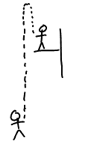
\includegraphics[scale=.8]{/Users/jgates/desktop/latex/pics/tokentoss.png}
%\end{floatingfigure}
 
{\bf \Large{\arabic{ProbNum}}} A cannon is shot straight up into the air. The cannonball leaves the cannon moving ${45~\tfrac{m}{s}}$.  

\bigskip  After how much time in the air will it have a speed of ${20~\tfrac{m}{s}}$? Use algebraic problem-solving.

%\begin{center}
%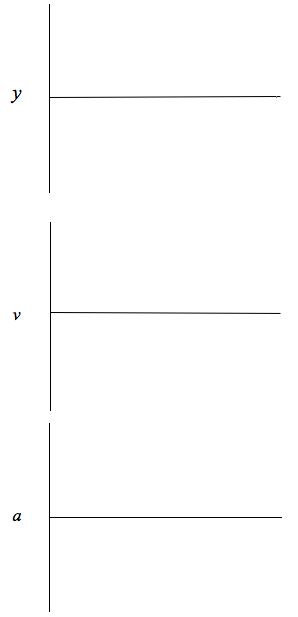
\includegraphics[scale=.85]{/Users/jgates/desktop/latex/pics/blankyvagraphstack.png}
%\end{center}


\vfill
\newpage